\documentclass[10pt,twocolumn,letterpaper]{article}

\usepackage{iccv}
\usepackage{times}
\usepackage{epsfig}
\usepackage{graphicx}
\usepackage{amsmath}
\usepackage{amssymb}
% Include other packages here, before hyperref.
\usepackage{url}
\usepackage{subfigure}
\usepackage{lineno}
% If you comment hyperref and then uncomment it, you should delete
% egpaper.aux before re-running latex.  (Or just hit 'q' on the first latex
% run, let it finish, and you should be clear).
\usepackage[pagebackref=true,breaklinks=true,letterpaper=true,colorlinks,bookmarks=false]{hyperref}

% \iccvfinalcopy % *** Uncomment this line for the final submission

\def\iccvPaperID{****} % *** Enter the ICCV Paper ID here
\def\httilde{\mbox{\tt\raisebox{-.5ex}{\symbol{126}}}}

% Pages are numbered in submission mode, and unnumbered in camera-ready
\ificcvfinal\pagestyle{empty}\fi
\begin{document}

%%%%%%%%% TITLE
\title{Patch Group Based Image Prior Learning for High Performance Denoising}

\author{First Author\\
Institution1\\
Institution1 address\\
{\tt\footnotesize firstauthor@i1.org}
% For a paper whose authors are all at the same institution,
% omit the following lines up until the closing ``}''.
% Additional authors and addresses can be added with ``\and'',
% just like the second author.
% To save space, use either the email address or home page, not both
\and
Second Author\\
Institution2\\
First line of institution2 address\\
{\tt\footnotesize secondauthor@i2.org}
}
\maketitle
%\thispagestyle{empty}

\begin{figure}
\centering
\subfigure{
\begin{minipage}{0.075\textwidth}
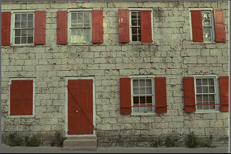
\includegraphics[width=1\textwidth]{24images/resize_kodim01.png}
\end{minipage}
\begin{minipage}{0.075\textwidth}
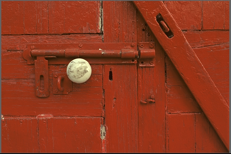
\includegraphics[width=1\textwidth]{24images/resize_kodim02.png}
\end{minipage}
\begin{minipage}{0.075\textwidth}
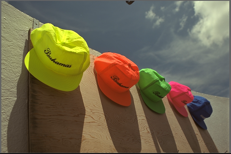
\includegraphics[width=1\textwidth]{24images/resize_kodim03.png}
\end{minipage}
\begin{minipage}{0.075\textwidth}
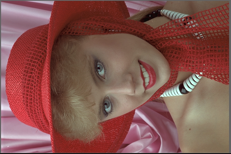
\includegraphics[width=1\textwidth]{24images/resize_kodim04.png}
\end{minipage}
\begin{minipage}{0.075\textwidth}
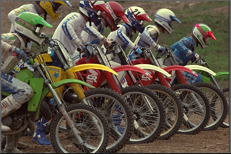
\includegraphics[width=1\textwidth]{24images/resize_kodim05.png}
\end{minipage}
\begin{minipage}{0.075\textwidth}
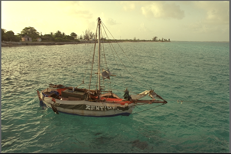
\includegraphics[width=1\textwidth]{24images/resize_kodim06.png}
\end{minipage}
}\vspace{-3mm}
\subfigure{
\begin{minipage}{0.075\textwidth}
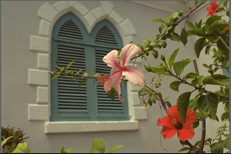
\includegraphics[width=1\textwidth]{24images/resize_kodim07.png}
\end{minipage}
\begin{minipage}{0.075\textwidth}
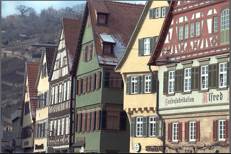
\includegraphics[width=1\textwidth]{24images/resize_kodim08.png}
\end{minipage}
\begin{minipage}{0.075\textwidth}
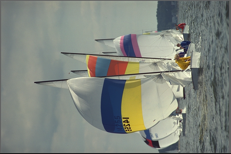
\includegraphics[width=1\textwidth]{24images/resize_kodim09.png}
\end{minipage}
\begin{minipage}{0.075\textwidth}
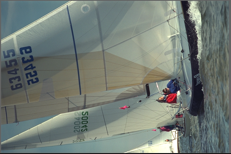
\includegraphics[width=1\textwidth]{24images/resize_kodim10.png}
\end{minipage}
\begin{minipage}{0.075\textwidth}
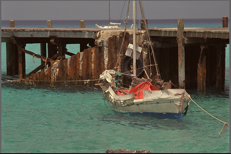
\includegraphics[width=1\textwidth]{24images/resize_kodim11.png}
\end{minipage}
\begin{minipage}{0.075\textwidth}
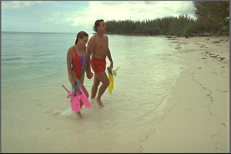
\includegraphics[width=1\textwidth]{24images/resize_kodim12.png}
\end{minipage}
}\vspace{-3mm}
\subfigure{
\begin{minipage}{0.075\textwidth}
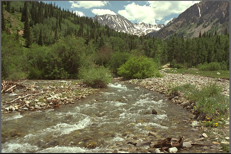
\includegraphics[width=1\textwidth]{24images/resize_kodim13.png}
\end{minipage}
\begin{minipage}{0.075\textwidth}
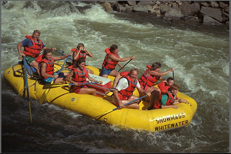
\includegraphics[width=1\textwidth]{24images/resize_kodim14.png}
\end{minipage}
\begin{minipage}{0.075\textwidth}
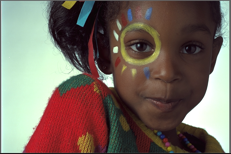
\includegraphics[width=1\textwidth]{24images/resize_kodim15.png}
\end{minipage}
\begin{minipage}{0.075\textwidth}
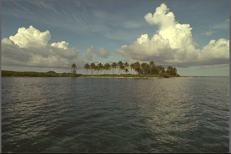
\includegraphics[width=1\textwidth]{24images/resize_kodim16.png}
\end{minipage}
\begin{minipage}{0.075\textwidth}
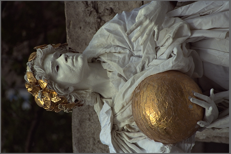
\includegraphics[width=1\textwidth]{24images/resize_kodim17.png}
\end{minipage}
\begin{minipage}{0.075\textwidth}
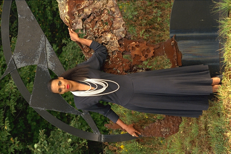
\includegraphics[width=1\textwidth]{24images/resize_kodim18.png}
\end{minipage}
}\vspace{-3mm}
\subfigure{
\begin{minipage}{0.075\textwidth}
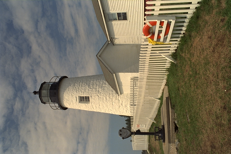
\includegraphics[width=1\textwidth]{24images/resize_kodim19.png}
\end{minipage}
\begin{minipage}{0.075\textwidth}
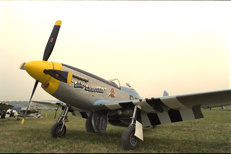
\includegraphics[width=1\textwidth]{24images/resize_kodim20.png}
\end{minipage}
\begin{minipage}{0.075\textwidth}
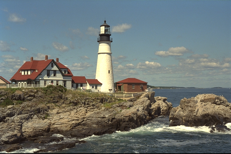
\includegraphics[width=1\textwidth]{24images/resize_kodim21.png}
\end{minipage}
\begin{minipage}{0.075\textwidth}
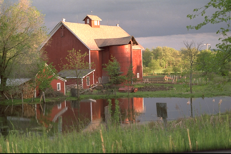
\includegraphics[width=1\textwidth]{24images/resize_kodim22.png}
\end{minipage}
\begin{minipage}{0.075\textwidth}
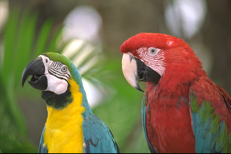
\includegraphics[width=1\textwidth]{24images/resize_kodim23.png}
\end{minipage}
\begin{minipage}{0.075\textwidth}
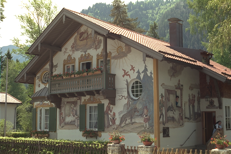
\includegraphics[width=1\textwidth]{24images/resize_kodim24.png}
\end{minipage}
}\vspace{1mm}
\caption{The 24 high quality color images from the Kodak PhotoCD Dataset.}
\label{f2}
\vspace{-2mm}
\end{figure}

Fig.\ \ref{f3} shows a scene denoised by the compared methods.\ We can see that the methods of CBM3D and NC would remain some noise on the recovered images. The methods of MLP, TNRD, and ``WNNM0'', which process separately the channels of color images, would over-smooth  the images and generate false colors or artifacts. The method ``WNNM1'', which process jointly the channels of color images, would not generate false colors, but still over-smooth the image. The ``WNNM2'', which is the WNNM model solved by ADMM algorithm, would remain some noise on the image.\ By employing the proposed MC-WNNM model, our method preserves the structures (e.g., textures in windows and grass) better across the R, G, B channels and generate less artifacts than other denoising methods, leading to visually pleasant outputs.\


\begin{figure*}\vspace{1mm}
\centering
\subfigure{
\begin{minipage}[t]{0.195\textwidth}
\centering
\raisebox{-0.15cm}{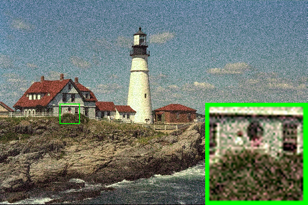
\includegraphics[width=1\textwidth]{comparea/resize_br_Noisy_nSig402030_kodim21.png}}
{\footnotesize (a) Noisy kodim21: 18.28dB }
\end{minipage}
\begin{minipage}[t]{0.195\textwidth}
\centering
\raisebox{-0.15cm}{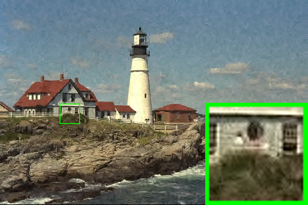
\includegraphics[width=1\textwidth]{comparea/resize_br_CBM3D_nSig402030_kodim21.png}}
{\footnotesize (b) CBM3D \cite{cbm3d}: 26.54dB}
\end{minipage}
\begin{minipage}[t]{0.195\textwidth}
\centering
\raisebox{-0.15cm}{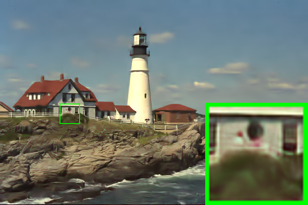
\includegraphics[width=1\textwidth]{comparea/resize_br_MLP_nSig402030_kodim21.png}}
{\footnotesize (c) MLP \cite{mlp}: 27.53dB}
\end{minipage}
\begin{minipage}[t]{0.195\textwidth}
\centering
\raisebox{-0.15cm}{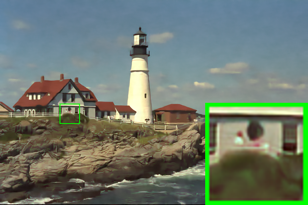
\includegraphics[width=1\textwidth]{comparea/resize_br_TNRD_nSig402030_kodim21.png}}
{\footnotesize (d) TNRD \cite{chen2015learning}: 27.60dB }
\end{minipage}
\centering
\begin{minipage}[t]{0.195\textwidth}
\raisebox{-0.15cm}{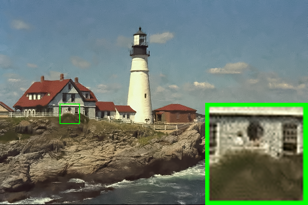
\includegraphics[width=1\textwidth]{comparea/resize_br_NC_nSig402030_kodim21.png}}
{\footnotesize (e) NC \cite{noiseclinic,ncwebsite}: 26.48dB  } 
\end{minipage}
}\vspace{-3mm}
\subfigure{
\begin{minipage}[t]{0.195\textwidth}
\centering
\raisebox{-0.15cm}{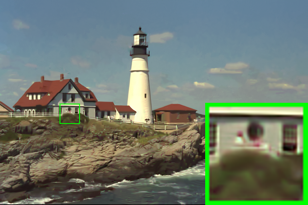
\includegraphics[width=1\textwidth]{comparea/resize_br_WNNMCW_nSig402030_kodim21.png}}
{\footnotesize (f) WNNM0: 27.80dB  }
\end{minipage}
\begin{minipage}[t]{0.195\textwidth}
\centering
\raisebox{-0.15cm}{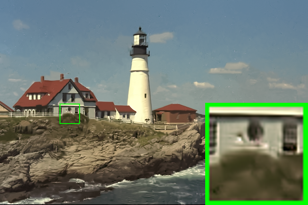
\includegraphics[width=1\textwidth]{comparea/resize_br_WNNMJ_nSig402030_kodim21.png}}
{\footnotesize (g) WNNM1: 27.75dB  }
\end{minipage}
\begin{minipage}[t]{0.195\textwidth}
\centering
\raisebox{-0.15cm}{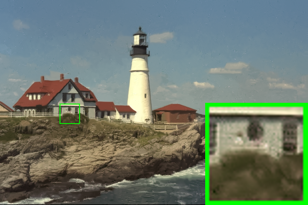
\includegraphics[width=1\textwidth]{comparea/resize_br_WNNM_ADMM_nSig402030_kodim21.png}}
{\footnotesize (h) WNNM2: 27.12dB }
\end{minipage}
\begin{minipage}[t]{0.195\textwidth}
\centering
\raisebox{-0.15cm}{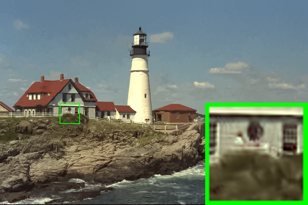
\includegraphics[width=1\textwidth]{comparea/resize_br_CWNNM_ADMM_nSig402030_kodim21.png}}
{\footnotesize (i) MC-WNNM: \textbf{28.34}dB}
\end{minipage}
\begin{minipage}[t]{0.195\textwidth}
\centering
\raisebox{-0.15cm}{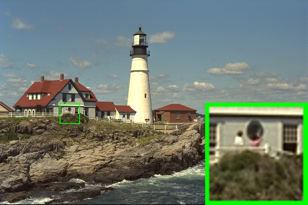
\includegraphics[width=1\textwidth]{comparea/resize_br_kodim21.png}}
{\footnotesize (j) Clean kodim21}
\end{minipage}
}\vspace{-0.5mm}
\caption{Denoised images of different methods on the image ``kodim21'' degraded by AWGN with different standard derivations of $\sigma_{r}=40, \sigma_{g}=20, \sigma_{b}=30$ on R, G, B channels, respectively. The images are better to be zoomed in on screen.}
\label{f3}
\vspace{-3mm}
\end{figure*}


\bibliographystyle{ieee}
\bibliography{egbib}

\end{document}
